\chapter{Diagnostics and goodness of fit}\label{ch:diagnostics}

A fit of \nwlsm{} is a sample from a posterior distribution, and two questions come before the interpretation: did the sampler converge, and does the model reproduce the network? Look at the chains first (\texttt{estat mcmcdiag}), then at the fit (\texttt{estat gof}, \texttt{estat ppcheck}), then read the results.

\section{Convergence: estat mcmcdiag}

\texttt{estat mcmcdiag} [\opt{nolist graph name(name)}] shows, for the coefficients, the log likelihood and the variance parameters, the posterior mean and standard deviation, the effective sample size, the Geweke $z$-score and, with several chains, the Gelman--Rubin statistic, and returns them in \texttt{r(diag)}.
\showlog{karate_diag}
The \emph{effective sample size} (ESS) says how many independent draws the correlated draws are worth; it is computed by the initial monotone positive sequence estimator of Geyer~\cite{geyer1992}. Here the 2,000 draws are worth between 160 and 260 independent draws, enough for the means but small for the tails of the intervals; a longer run (\opt{nsample()}, \opt{interval()}) raises it. With several chains the ESS is the sum over the chains. A warning is printed when the smallest ESS is below 100: run longer before reading the estimates. The smallest ESS is returned in \texttt{r(ess\_min)}, and \texttt{r(ess\_flag)} is 1 when the warning was shown. The \emph{Gelman--Rubin statistic} (Rhat)~\cite{gelman1992} compares the chains with each other: values close to 1, say below 1.1, indicate that they agree. Run at least two chains for results that matter, and look at these numbers before looking at anything else. The acceptance rates of the random-walk steps are shown below the table; they should be near the tuning target of 0.234.

\paragraph{The Geweke $z$-score.} The Geweke $z$-score~\cite{geweke1992} compares the mean of the first 10\% of the draws of a chain with the mean of its last 50\%. It is computed as \texttt{geweke.diag(x, frac1 = 0.1, frac2 = 0.5)} of the R package \texttt{coda} computes it, for every parameter and every chain: $z=(\bar x_1-\bar x_2)/\sqrt{s_1/n_1+s_2/n_2}$, where $s_1$ and $s_2$ are the spectral densities at frequency zero of the two parts, each estimated from an autoregressive fit as \texttt{spectrum0.ar()} does. The $z$ of a series that does not move is missing (R gives NaN) and is left out of the counts. The Geweke column of the main table shows, for every row, the $z$ of largest size over the chains (the $z$ itself with one chain). With 2 to 8 chains a second table shows the $z$ of every chain, as R prints it.

The Geweke $z$ is informational: it is not a test of convergence. The footnote under the table counts how many of the $k$ values (parameters times chains) exceed 1.96 in size and says that about $0.05\,k$ are expected to do so by chance with long settled chains. With short chains the first part has only a few dozen draws, its spectral density is noisy, and more values exceed 1.96, so 1.96 is the nominal limit of a two-sided 5\% test only in the long-chain case and no verdict is given. Read the $z$ values together with the trace plots and the effective sample sizes. The values are returned in \texttt{r(geweke\_z)} (chains by parameters), the largest size in \texttt{r(geweke\_max)}, the number of values in \texttt{r(geweke\_ntests)} and the number above 1.96 in \texttt{r(geweke\_nexceed)}.

A single large $z$ among many parameters can happen by chance: in the fit with sender and receiver effects of the Lazega network, the Geweke $z$ of the sender variance is $-2.42$ in the second chain (the footnote counts 1 of 10 values above 1.96, where 0.5 would be expected), while its Gelman--Rubin statistic is 1.000 and its ESS 1,508 of 4,000:
\showlog{lazega_diag}
\paragraph{Trace plots.} With \opt{graph} the trace plots of all these quantities are drawn, one line per chain, with the Gelman--Rubin statistic in the title, and combined into one graph.
\begin{figure}[ht]\centering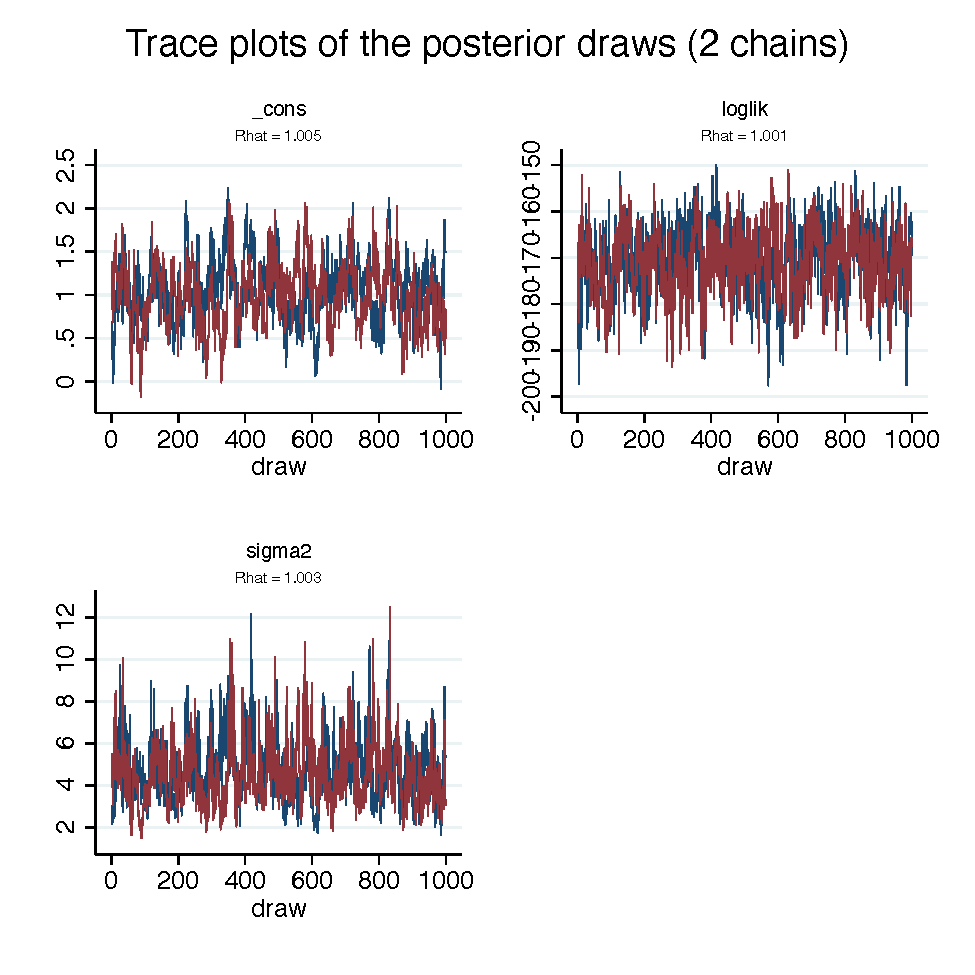
\includegraphics[width=0.9\textwidth]{fig/fig_karate_trace.pdf}
\caption{\texttt{estat mcmcdiag, graph}: trace plots of the two chains of the karate club fit.}\end{figure}

\section{Goodness of fit: estat gof}

\texttt{estat gof} is the goodness of fit of \latentnet{}'s \texttt{gof()}: one network is simulated from the model at each of \opt{nsim()} posterior draws (default 100), taken evenly spaced from the stored draws, and statistics of the observed network are compared with their distribution over the simulated networks. The simulation is done natively, independent of \opt{threads()}. \opt{gof(terms)} lists the statistics: \texttt{degree} (undirected), \texttt{idegree} and \texttt{odegree} (directed), \texttt{espartners} (edgewise shared partners; for directed networks the outgoing two-paths $i\to k\to j$), \texttt{dspartners} (dyadwise shared partners), \texttt{distance} (geodesic distances; the last cell is the unreachable pairs), \texttt{model} (the total value of the ties and the sum of each covariate over the ties) and \texttt{values} (valued networks: the number of dyads with each value; for the normal family in ten bins of equal observed frequency). The default is \latentnet{}'s: \texttt{degree distance} (undirected) or \texttt{idegree odegree distance} (directed), plus \texttt{values} for the Poisson and binomial families, and \texttt{model values} for the normal family. \opt{seed()}, \opt{maxdeg()}, \opt{maxdist()} and \opt{cutoff()} (Chapter~\ref{ch:valued}) are the other options.
\showlog{karate_gof}
For each cell the table shows the observed count, the minimum, mean and maximum over the simulated networks and the Monte Carlo $p$-value $2\min(P(\text{simulated}\le\text{observed}),P(\text{simulated}\ge\text{observed}))$, at most 1, as in \latentnet{}. In the karate club the distance model reproduces the geodesic distances well (all $p$-values above 0.05), but not the degrees: the club has 11 members with exactly two friends, where the simulated networks have 3.6 on average ($p<0.005$), and the two members with 16 and 17 friends are reproduced by hardly any simulated network ($p=0.02$ and 0.00). A model with the random \opt{sociality} effect is the natural next step for such hubs (Chapter~\ref{ch:effects}). Missing dyads of the observed network count as no tie.

For a directed network with latent clusters (Sampson's monks, Chapter~\ref{ch:clusters}) the table of out-degrees shows that 16 of the 18 monks name exactly three others, where the model implies 4.5 on average ($p=0.00$) and expects some monks with two (4.2) or fewer, which none has:
\showlog{monks_gof}
\begin{figure}[ht]\centering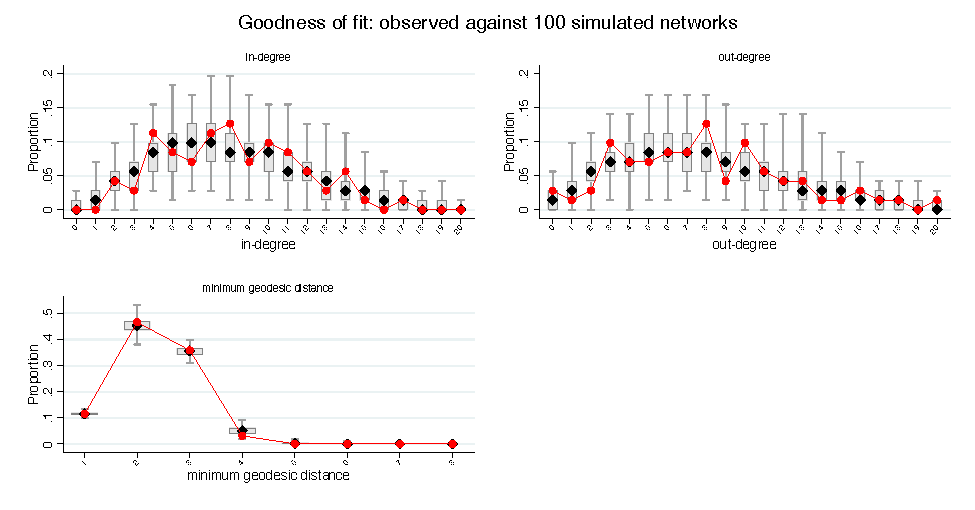
\includegraphics[width=\textwidth]{fig/fig_lazega_gof.pdf}
\caption{\texttt{estat gof, plot maxdeg(20) maxdist(8)} for the Lazega friendship network with sender and receiver effects: the shares of the observed network (red line) and of the simulated networks (box plots) for the in-degrees, out-degrees and geodesic distances.}\end{figure}
With \opt{plot} the shares of the observed and the simulated networks are drawn in box plots, the observed network as a red line.

\section{Calibration: estat ppcheck}

\texttt{estat ppcheck} [\opt{groups(\#) graph name(name) nolist}] is a posterior predictive check of the tie probabilities: the dyads are sorted by their posterior mean predicted probability (expected value) and cut into \opt{groups()} groups of about equal size (default 10); the table compares the mean prediction with the observed mean in every group. Below it come, for binary networks, the Brier score, the area under the ROC curve (AUC) and the mean log loss, and for valued networks the root mean squared error, the correlation and the mean absolute error of the posterior mean expected values with the observed values. \opt{graph} draws the calibration plot. The results are in \texttt{r(groups)}, \texttt{r(score)}, \texttt{r(auc\_or\_corr)} and \texttt{r(N)}.
\showlog{karate_ppcheck}
In the karate club the AUC is 0.96: the model ranks the observed ties far above the non-ties. The last group has a predicted mean of 0.37 and an observed mean of 0.88, which says that the model is not confident enough about the most probable ties. The Brier score is 0.080.
\begin{figure}[ht]\centering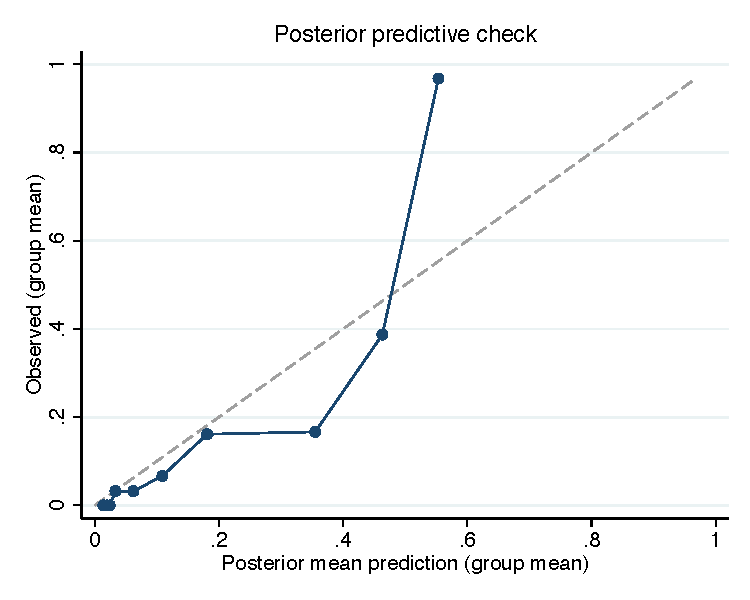
\includegraphics[width=0.7\textwidth]{fig/fig_monks_ppcheck.pdf}
\caption{\texttt{estat ppcheck, graph} for the monks network with three clusters: observed against predicted mean by group.}\end{figure}
